\documentclass[9pt,twocolumn,twoside]{pnas-new}
% DTU 02805 final project. Written into the PNAS Overleaf template the course asks for:
% https://www.overleaf.com/latex/templates/template-for-preparing-your-research-report-submission-to-pnas-using-overleaf/fzcbzjvpvnxn
% Figures: paper/make_figures.py. References: paper/references.bib (also listed in docs/overview/literature.pdf).
% DRAFT 14 Nov 2026. Lines marked TODO need the group.

\articletype{Social Sciences}
\templatetype{pnasresearcharticle}
\graphicspath{{figures/}}

\begin{document}

\title{Who makes a film predicts its return; what its script says does not}

\author[a]{\`{A}ngela Bux\'{o}}
\author[a]{Gyula K\"{u}rthy}
\author[a]{Niklas Johansen}
\affil[a]{Technical University of Denmark (DTU), 02805 Social Graphs and Interactions, Kgs.\ Lyngby, Denmark}

\leadauthor{Bux\'{o}}

\significancestatement{Studios bet hundreds of millions on films whose returns are famously hard to foresee. We ask which kind of information actually carries signal about a film's return on its budget: the network of people and companies who made it, the text of its screenplay, or how critics and audiences received it. Tested on films released after the model was fitted, the collaboration network carries most of the pre-release signal, while the words and the emotional shape of the screenplay add nothing once budget, genre and era are known.}

\authorcontributions{TODO (the course asks for specific roles; confirm before hand-in). Draft: G.K. built the data pipeline, the movie graph, the profit model, the return-similarity test and the two screenplay text analyses; \`{A}.B. built the review analysis (critics, audiences and money); N.J. built the actor co-appearance network and its interactive explorer. All authors wrote the paper. Hand labelling: TODO.}
\authordeclaration{The authors declare no competing interests.}
\correspondingauthor{\textsuperscript{1}To whom correspondence should be addressed. TODO e-mail.}

\keywords{box office $|$ collaboration networks $|$ screenplays $|$ sentiment arcs $|$ film critics}

\begin{abstract}
What predicts whether a film earns back its budget, and does earning agree with being liked? We combine IMDb, Wikipedia and Wikidata into one network of 12,673 films and the people and companies behind them, add 1,095 screenplays and audience reviews, and measure return as $\ln(\text{gross}/\text{budget})$. Trained on films to 2010 and tested on 2011--2017, budget, year and genre explain nothing ($R^2=-0.01$), and adding leakage-safe network track records raises $R^2$ to 0.20. Films sharing a producer, writer or studio have more similar returns than shuffles allow (0.09--0.17 against at most 0.02). Screenplay text adds nothing: the words of profitable and unprofitable scripts differ only through franchise films, and two pre-registered emotional-arc tests are null ($\rho=0.035$, $p=0.32$) or a near miss ($\rho=0.078$, $p=0.028$, threshold 0.025). Critics and audiences agree with money only moderately ($\rho\approx0.3$).
\end{abstract}

\dates{This manuscript was compiled on \today}
\doi{DTU 02805 final project, autumn 2026}

\maketitle
\thispagestyle{firststyle}
\ifthenelse{\boolean{shortarticle}}{\ifthenelse{\boolean{singlecolumn}}{\abscontentformatted}{\abscontent}}{}

\Firstpage

\dropcap{F}ilm returns are heavy-tailed and notoriously hard to predict~\cite{devany1999uncertainty}. Three kinds of information are available about a film, and each has its own literature. The first is \emph{who made it}: careers and collaboration networks shape creative success~\cite{uzzi2005collaboration,cattani2008core,ferriani2009relational}, stars raise revenue without raising returns~\cite{ravid1999information,elberse2007power}, and past collaborations predict profitability~\cite{lash2016early,packard2016network}. The second is \emph{what the film says}: script text has been used to green-light films~\cite{eliashberg2007story,eliashberg2014assessing,hunter2016predicting}, and the emotional arc of a story has been linked to success~\cite{reagan2016emotional,delvecchio2021improving,toubia2021quantifying,berger2021engaging}. The third is \emph{how it was received}: critics predict more than they drive revenue~\cite{eliashberg1997critics,basuroy2003critical,reinstein2005influence}, and critical taste and market success can part ways~\cite{holbrook1999popular,holbrook2007taste,holbrook2008art}.

These strands are rarely tested side by side, on the same films, against the same outcome. Most studies model revenue, which budget largely determines; we model the \emph{multiple}, $\ln(\text{worldwide gross}/\text{budget})$, the return on the reported budget. We ask which strand carries signal about it, and whether that signal survives the checks that rule out the boring explanations: budget, genre and era, franchise membership, and leakage from the future. The short answer is that the network does, the screenplay does not, and reception agrees with money only in part.

\section*{Results}

\subsection*{The collaboration network carries the pre-release signal}
We fit ridge regressions on films released up to 2010 and score them on films from 2011 to 2017, so no later film informs a prediction. Budget, year and genre alone explain none of the variance in the multiple out of sample ($R^2=-0.010$; Fig.~\ref{fig:network}A). Adding the track records, experience and centrality of each film's studio, distributor, producers, writers, director and top-billed cast, all computed only from earlier films, raises $R^2$ to 0.202. Release month and a franchise flag add little more (0.244). Critic and audience scores raise it to 0.312, but they are known only after release and are reported as reception, not prediction. The strongest single network measure is the studio's track record ($\rho=+0.27$ with the multiple, net of budget and year; 4,568 films). A director's next film is a hit (top quarter) 35\% of the time after a hit and 18\% after a non-hit. Shuffling the order of each director's own films leaves about half that gap (0.090 of 0.175), so roughly half reflects lasting differences between directors and the rest momentum or era, in line with hot streaks in creative careers~\cite{liu2018hot,john2017managerial}. PageRank in yearly collaboration networks adds nothing beyond plain experience counts ($\rho=-0.003$).\Endparasplit

Returns also cluster by shared personnel (Fig.~\ref{fig:network}B). For every role, films sharing a person or company have more similar residual returns than 1,000 shuffles allow: from 0.09 for the top-three cast to 0.17 for producers, against a 95th null percentile of at most 0.02. The pattern holds without franchise films (0.07--0.14), with ranked returns (0.08--0.16) and from 1980 on (0.09--0.16). Roles overlap, since a director's films often share a studio, so we also shuffled only within each film's main studio: about half of each people role's similarity survives.

\begin{figure*}
\centering
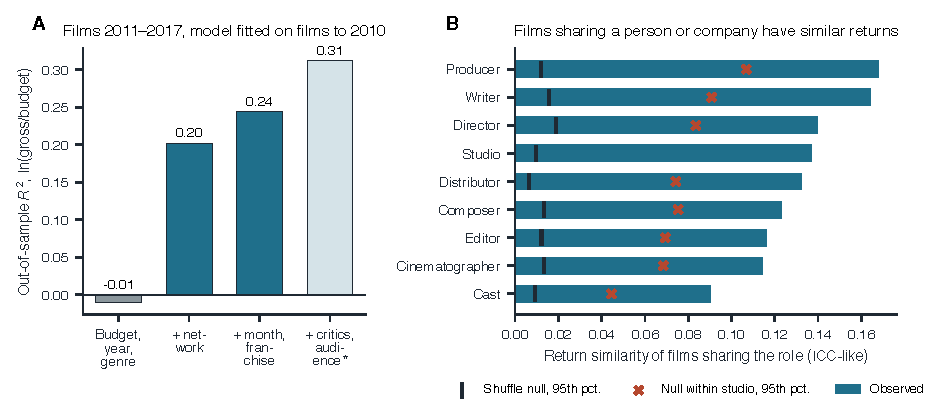
\includegraphics[width=\textwidth]{fig_network.pdf}
\caption{Who made a film carries signal about its return. (A) Out-of-sample $R^2$ for $\ln(\text{gross}/\text{budget})$ on films from 2011--2017, from ridge models fitted on films to 2010; network features use only films released earlier. *Critic and audience scores are known only after release. (B) Return similarity (an intraclass-correlation-like share of residual variance, after $\ln$ budget, decade and genre) among films sharing each role, 6,851 films. Bars: observed; black ticks: 95th percentile of 1,000 shuffles that keep every group's size; red crosses: the same null when returns are shuffled only within a film's main studio.}
\label{fig:network}
\end{figure*}

\subsection*{The screenplay adds nothing once budget, genre and era are known}
We compared the dialogue of the most and least profitable quarter of 1,095 scripts within genre $\times$ decade cells, with a log-odds score~\cite{monroe2008fightin,kessler2017scattertext} fixed before seeing results. The number of distinctive words is only slightly above a stratified shuffle null ($z=2.08$, $p=0.024$; Fig.~\ref{fig:script}A). In the franchise check, which uses 200 shuffles per run, the same comparison gives $z=2.05$ with all films and $z=0.50$ without the 93 likely franchise films, while removing the same number of random films never falls that low (0 of 50 draws; median $z=2.94$). The excess goes with the franchise films themselves; we did not test why. A TF-IDF classifier on the words does no better than genre, decade and budget (AUC 0.58 against 0.58).

The emotional arc fares no better. We scored every sentence of 834 non-franchise scripts with DistilBERT fine-tuned on SST-2~\cite{sanh2019distilbert}, built a 100-point arc per film, and pre-registered two descriptors: its swing (D1, the SD of the smoothed arc) and its ending lift (D2, last fifth minus first fifth). With genre $\times$ decade cells, $\ln$ budget and scene length partialled out of both sides, swing is unrelated to return ($\rho=0.035$, 95\% CI $[-0.03, 0.11]$, $p=0.32$) and ending lift is a near miss ($\rho=0.078$, $[0.01, 0.15]$, $p=0.028$ against a Bonferroni threshold of 0.025; Fig.~\ref{fig:script}B). Adding the arc to a cross-validated model does not improve it ($\Delta R^2=-0.002$). Split-half reliability of the descriptors is about 0.45, so roughly half of their between-film variance is scene-level noise.

One study reports that ``Man in a hole'' arcs earn more~\cite{delvecchio2021improving}. We rebuilt its pipeline on our arcs (low-pass smoothing, six $k$-means shapes, one regression of revenue on each shape's dummy). Their headline effect does not reproduce, even in their specification (VADER~\cite{hutto2014vader}: $+\$9$M, $p=0.67$; SST-2: $+\$24$M, $p=0.32$). Their specification does yield a different ``finding'' in our data, a lower revenue for one shape ($p=0.015$), which disappears with our outcome and controls. This is exploratory and not pre-registered.

\begin{figure}
\centering
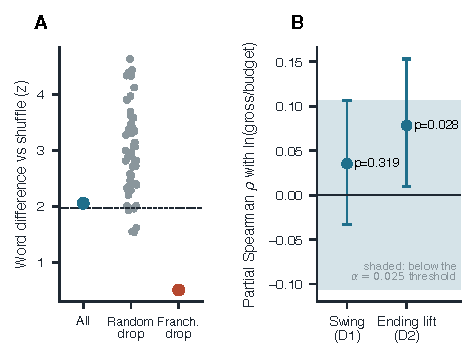
\includegraphics[width=\linewidth]{fig_script.pdf}
\caption{The screenplay's words and arcs show no robust link to return. (A) Excess of distinctive words between the top and bottom quarter of scripts by return, as $z$ against a genre $\times$ decade shuffle (200 shuffles per run): all 526 labelled films, 50 drops of 93 random films, and the drop of the 93 likely franchise films. Dashed: $z=1.96$. (B) Pre-registered partial Spearman correlation of the arc's swing and ending lift with $\ln(\text{gross}/\text{budget})$, 834 films, with 95\% bootstrap intervals; shaded: correlations too small to pass the Bonferroni threshold.}
\label{fig:script}
\end{figure}

\subsection*{Critics and audiences agree with money only in part}
On 2,095 films up to 2017, the multiple correlates with the IMDb rating at $\rho=0.27$, Metacritic at 0.26 and Rotten Tomatoes at 0.33, all far above a null that shuffles within genre $\times$ decade, which itself sits near 0.1 (Fig.~\ref{fig:reception}). Critics agree with each other far more (Metacritic with Rotten Tomatoes, 0.93) than with money. The tone of audience reviews (VADER, first 50 Tag Genome reviews~\cite{vig2012tag}) tracks the multiple weakly (0.13). Ranking films by rating minus money separates films ``liked beyond their money'', whose reviews mention auteurs and \emph{noir}, from films that ``earned beyond their liking'', whose reviews mention \emph{scares} and \emph{slashers}: cheap horror earns its budget back without being loved. Over the full clean sample there are 158 critically loved flops and 205 panned hits.

\begin{figure}
\centering
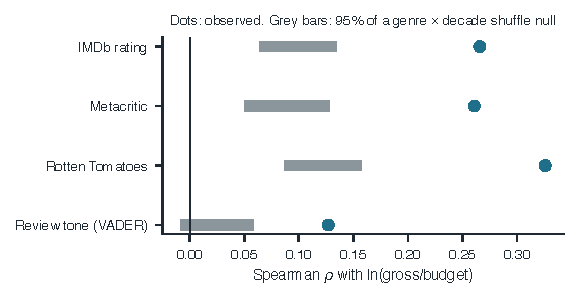
\includegraphics[width=\linewidth]{fig_reception.pdf}
\caption{Being liked and making money agree only in part. Spearman correlation of each reception measure with $\ln(\text{gross}/\text{budget})$ on 2,095 films up to 2017 (dots), against 95\% of a null that shuffles the outcome within genre $\times$ decade cells (grey bars). The null is not centred on zero because genre and era alone align reception and return.}
\label{fig:reception}
\end{figure}

\section*{Discussion}
Across three kinds of information, the one that predicts a film's return before release is who made it. Track records carry most of that signal, and network position adds little beyond experience, in line with work that found network effects weaken once budget is known~\cite{packard2016network} and that stars buy revenue, not returns~\cite{ravid1999information,elberse2007power}. The screenplay, by contrast, shows no robust link once budget, genre, era and franchise are handled. This agrees with the controlled study of emotional dynamics~\cite{berger2021engaging} and contradicts claims built on revenue without those controls~\cite{delvecchio2021improving}. The outcome matters: one study of revenue found critics' scores falling as box office rose~\cite{holbrook2007taste}, while against return on budget they rise, which suggests critics favour cheaper films that earn their budgets back.

What this does not show. None of these results is causal. Gross over budget is not profit, since marketing and the cinemas' share are missing. The return-similarity test uses all years at once and so describes clustering rather than prediction. A sentiment score measures what a classifier does on screenplay sentences, not what the audience feels; the arc descriptors are only moderately reliable, which caps any association, and we have not yet validated them against hand labels (TODO: report agreement once the sheets are filled). The 100k-vote sample under-represents flops, reviews stop in 2017, and the franchise flag is rough. A negative result is only as strong as its power: our arc test was powered for correlations of about 0.11, so smaller effects remain possible.

\matmethods{
\subsection*{Data}
Movies with at least 10,000 IMDb votes (non-adult) from IMDb's public files, linked to Wikipedia and Wikidata (TODO: collection dates). Budget and gross come from Wikipedia infoboxes; we keep films with both in US dollars and at least \$1,000, no rentals-only or regional gross, no streaming distributor and release before 2026 (6,851 films; 2,446 with 100,000+ votes). Screenplays are MovieSum~\cite{saxena2024moviesum} (1,095 clean films with 100,000+ votes); audience reviews are the MovieLens Tag Genome~\cite{vig2012tag} (2,070 films, none after 2017); critic scores come from Wikipedia and Wikidata. Franchise films are flagged from Wikidata (follows, followed by, part of a series).

\subsection*{The movie graph and network features}
An undirected bipartite graph links films to people (actors with billing order, directors, writers, producers, composers, cinematographers, editors) and companies (studios and distributors, merged through Wikidata identifiers). For each film, each role's experience, track record (mean multiple of earlier films) and PageRank in a collaboration network rebuilt per release year use only films released before it. Company communities: Louvain~\cite{blondel2008fast} on the company co-credit projection (1980--2017), ten seeds.

\subsection*{Prediction and similarity}
Ridge regressions with blocks added in turn; fitted on films to 2010 and scored on 2011--2017. Return similarity: for each role, the share of residual variance (after $\ln$ budget, decade and genre) explained by group membership among people or companies credited on at least two films; null: 1,000 shuffles of returns across films, keeping group sizes and overlaps; a second null shuffles only within main studio.

\subsection*{Screenplay text}
Dialogue only, character names removed, stopwords kept; terms in at least five scripts; score $\log_{10}$ of smoothed rate ratios with threshold $\log_{10}2$; 1,000 shuffles of the success label within genre $\times$ decade. Classifier: TF-IDF logistic regression, $10\times5$-fold cross-validation, against genre, decade and $\ln$ budget.

\subsection*{Emotional arcs}
Pre-registered before any sentiment was computed (config committed with the code). Scenes from screenplay markup; each sentence scored as $P(\text{pos})-P(\text{neg})$ by DistilBERT SST-2, chosen by a pre-set rule over VADER; scene score is the mean of its sentences; arcs resampled to 100 points and smoothed over 11. Primary test: partial Spearman (Frisch--Waugh residuals on genre $\times$ decade cells, $\ln$ budget and mean sentences per scene), 1,000 within-cell permutations, 2,000 bootstrap resamples, Bonferroni $\alpha=0.025$ for two descriptors. Robustness across three further sentiment models, layers, windows, samples and seeds is reported in the repository.

\subsection*{Reception}
Spearman correlations against 1,000 shuffles of the outcome within genre $\times$ decade (first-listed genre). Review tone: mean VADER compound score of a film's first 50 reviews; VADER agrees with Stanford polarity labels on 73\% of 1,988 non-neutral reviews. TODO: hand-labelled sample of 50 reviews.

\subsection*{Validation and availability}
Every analysis is compared with a shuffle null and, where possible, a second method. Code, configuration and numeric outputs are in the group repository (TODO: link); raw data, script and review text are not redistributed, in line with their licences.
}

\showmatmethods{}

\dataavail{Code, configuration files and all numeric outputs are in the group repository (TODO: public link). Raw IMDb files, screenplay text and review text are not redistributed, in line with their terms and licences; scripts to rebuild every input from the public sources are included.}

\acknow{TODO.}
\showacknow{}

\bibsplit[3]
\bibliography{references}

\end{document}
